\subsection{Snow}

The function \texttt{combnsnow()} accepts the same input arguments as the original function \texttt{combn()} from the CRAN package. \texttt{combnsnow()} can also handle the same types of valid inputs (see Section 2.1).\\
\null
Usage:\\
\null

\texttt{combnsnow <- function(cls, x, m, fun = NULL, simplify = TRUE, ...)}\\
\null

where \texttt{cls} is the clusters, \texttt{x} is the input vector of integers and/or characters, \texttt{m} is number of elements per combination
\texttt{fun} is the function to be applied to the resulting output, \texttt{simplify} indicates whether the output must be printed as a matrix (set to \texttt{TRUE}) or as a list (set to \texttt{FALSE}), and \texttt{...} are the parameters for \texttt{fun}.\\

\null
Code highlights:\\
\begin{itemize}
\item Load balancing algorithm implemented in R Snow
\end{itemize}
Other notes:
\begin{itemize}
\item Again, the program terminates if R decides that it cannot allocate enough space for the program to successfully run.
\end{itemize}

\subsubsection{The Issue of Communication Overhead}
After running tests using small inputs, it was observed that parallelization using Snow more often than not took longer than running the CRAN function \texttt{combn()}. This is because of the communication overhead. The communication between the nodes in the cluster took more time than the actual computations in the function. If the jobs sent to the worker nodes are not relatively computationally extensive, the overhead of communicating ends up deteriorating the performance.

\subsubsection{Reducing Network Overhead}
Communication is much slower than computation. There is already communication overhead to setting up clusters. In order to reduce network overhead and improve the performance, the code was written so that the nodes will do long calculations, and the tasks are going to be pre-assigned so that there will be less communications among the nodes as each work on its own tasks. The same load balancing algorithm as in Section 3.1.1 was used to distribute the tasks to each nodes.

\subsubsection{Comparative Analysis}
The same input sizes and function arguments as in Section 3.1.5 were used for testing. For the Snow tests, 8 clusters were used. The following plot illustrates the differences in speeds between the Snow and CRAN implementations:\\
\null

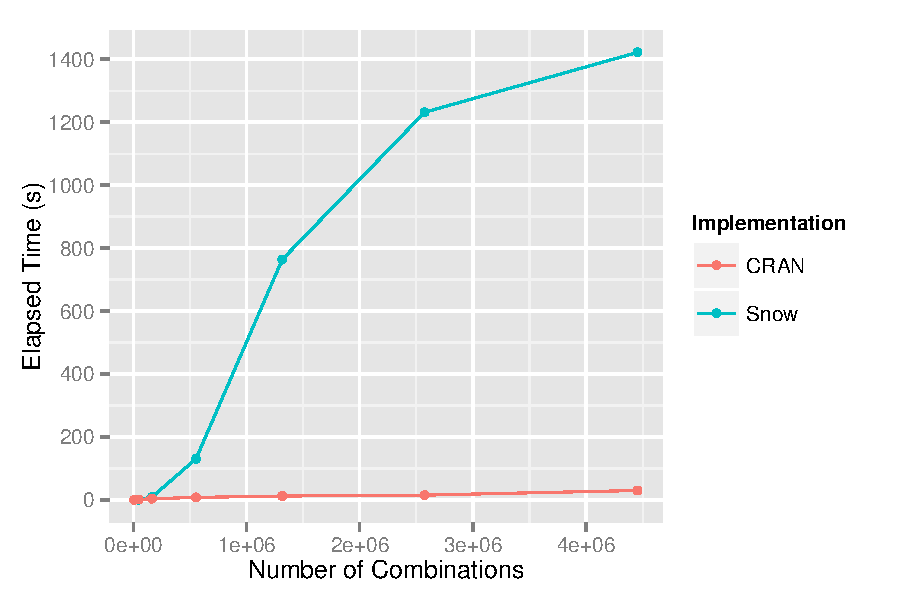
\includegraphics{snow.pdf}\\
\null

Despite our efforts to achieve speedups, the Snow implementation was actually much slower than the serial implementation of \texttt{combn()}. While the load balancing algorithm helped in distributing the tasks, there are other aspects in the code that makes the program slower. For instance, sorting and formatting of the output is not in parallel, which can take a really long time in R when the input size is really big. There is also the inevitable communication overhead due to the use of clusters.






